\begin{figure*}[ht]
  \centering
  \begin{subfigure}[b]{0.3\textwidth}
    \centering
    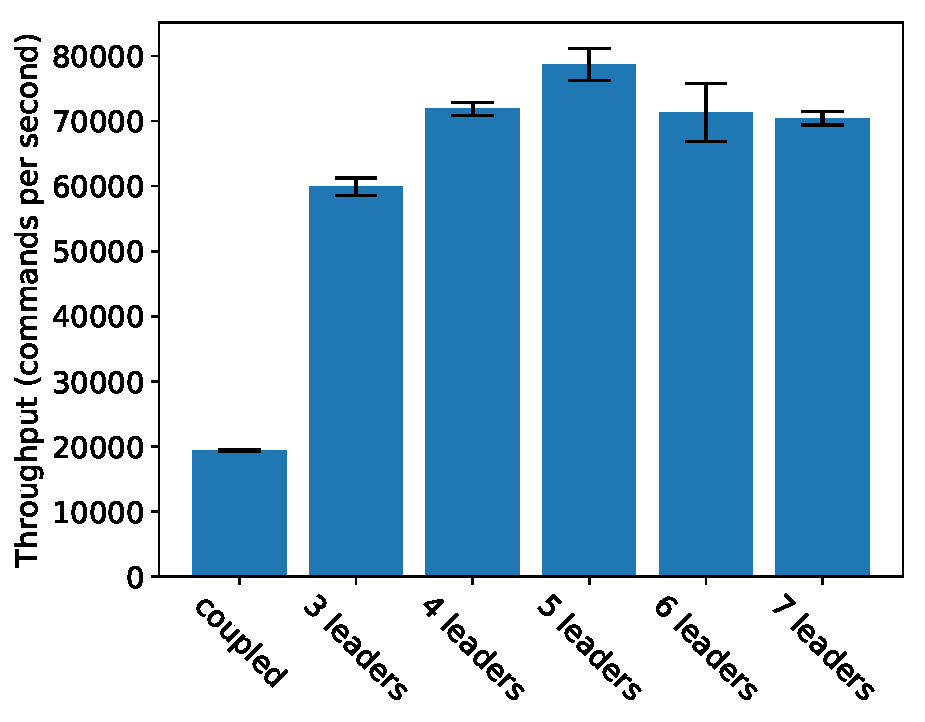
\includegraphics[width=\textwidth]{assets/nsdi_fig2_ablation_high_load_throughput.pdf}
    \caption{Throughput with 600 clients.}%
    \figlabel{EvalAblationHighLoadThroughput}
  \end{subfigure}\hspace{0.03\textwidth}
  \begin{subfigure}[b]{0.3\textwidth}
    \centering
    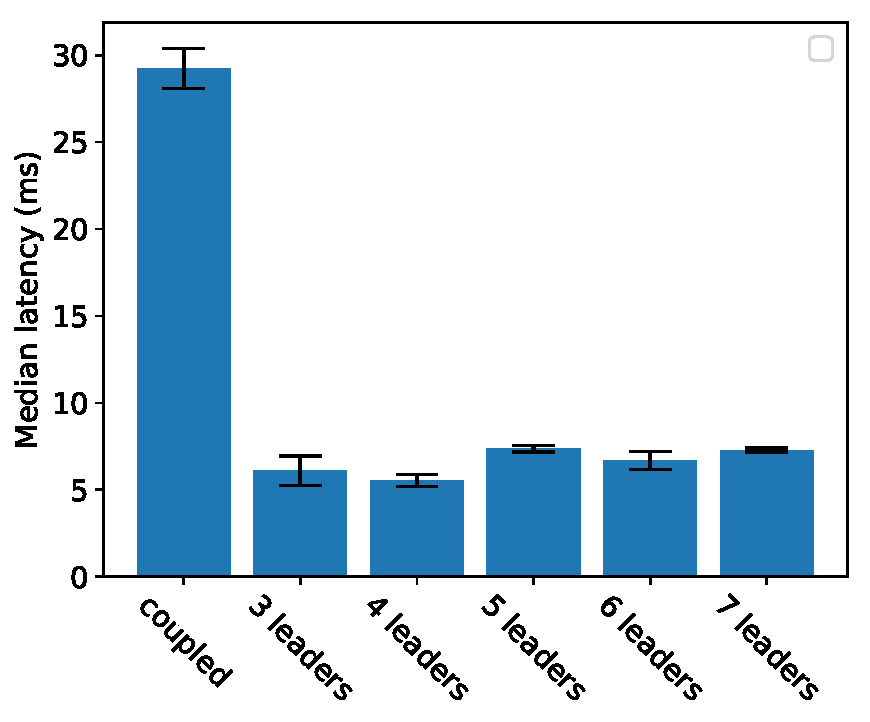
\includegraphics[width=\textwidth]{assets/nsdi_fig2_ablation_high_load_latency.pdf}
    \caption{Median latency (ms) with 600 clients.}%
    \figlabel{EvalAblationHighLoadLatency}
  \end{subfigure}\hspace{0.03\textwidth}
  \begin{subfigure}[b]{0.3\textwidth}
    \centering
    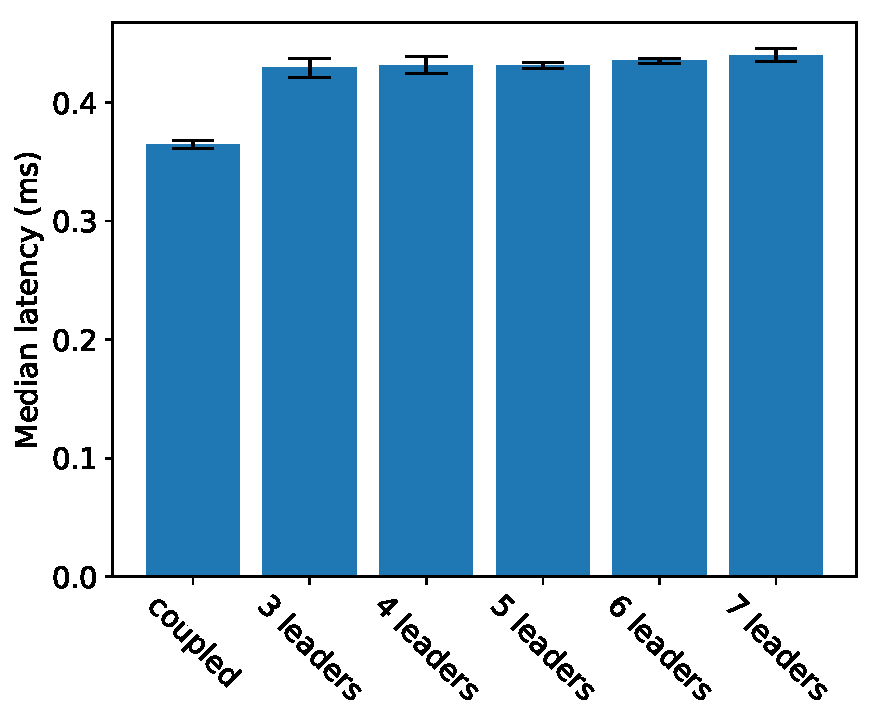
\includegraphics[width=\textwidth]{assets/nsdi_fig2_ablation_low_load_latency.pdf}
    \caption{Median latency (ms) with one client.}%
    \figlabel{EvalAblationLowLoadLatency}
  \end{subfigure}
  \caption{%
    An ablation study showing the effect of disaggregation and scaling on
    throughput and latency with 600 clients and one client. Throughput for one
    client is not shown because it is simply the inverse of latency.
  }\figlabel{EvalAblation}
\end{figure*}
